%%%%%%%%%%%%%%%%%%%%%%%%%%%%%%%%%%%%%%%%%%%%%%%%%%%%%%%%%%%%%%%%%%%%%%%%%%
%%%%%                         CHAPITRE 6                            %%%%%%
%%%%%%%%%%%%%%%%%%%%%%%%%%%%%%%%%%%%%%%%%%%%%%%%%%%%%%%%%%%%%%%%%%%%%%%%%%

\lhead[\fancyplain{}{\leftmark}]%Pour les pages paires \bfseries
      {\fancyplain{}{}} %Pour les pages impaires
\chead[\fancyplain{}{}]%
      {\fancyplain{}{}}
\rhead[\fancyplain{}{}]%Pour les pages paires 
      {\fancyplain{}{\rightmark}}%Pour les pages impaires \bfseries
\lfoot[\fancyplain{}{}]%
      {\fancyplain{}{}}
\cfoot[\fancyplain{}{\thepage}]%\bfseries
      {\fancyplain{}{\thepage}} %\bfseries
\rfoot[\fancyplain{}{}]%
     {\fancyplain{}{\scriptsize}}


%%%%%%%%%%%%%%%%%%%%%%%%%%%%%%%%%%%%%%%%%%%%%%%%%%%%%%%%%%%%%%%%%%%%%%%%%%
%%%%%                      Start part here                          %%%%%%
%%%%%%%%%%%%%%%%%%%%%%%%%%%%%%%%%%%%%%%%%%%%%%%%%%%%%%%%%%%%%%%%%%%%%%%%%%

\chapter{Using consumer-grade hardware - Application to boxing}
\label{ch:6}

%%% TITRE ARTICLE
%%% Evaluation of kinematic performance indicators in boxing in suboptimal conditions
%%% TITRE



%==============================================================================	Résumé du chapitre

\begin{center}
\rule{0.7\linewidth}{.5pt}
\begin{minipage}{0.7\linewidth}
\smallskip

\textit{In the context of a competition, research-grade hardware is not always workable as it is cumbersome and complex to set up. We tested the use of GoPro cameras, which are lightweight, but not straight-forward to calibrate or synchronize. We post-calibrated them on geometric cues, and post-synchronized them by correlation of keypoint speeds. The workflow was applied to shadow-boxing, which involves fast, 3 dimensional, and full-body movements. \newline\newline
The objective of the study was to verify whether it is possible to accurately measure Key Performance Indicators (KPIs) in boxing, with a markerless protocol using consumer-grade action cameras. This was concurrently validated with a marker-based protocol. A secondary goal was to compare the impact of resorting to post-calibration and post-synchronization, to choosing a more standard, less refined 2D pose estimation model. We conclude that KPIs are remarkably well evaluated in all conditions. Using a different 2D pose estimation model had a similar, but mild impact, on results, but combining both factors lead to more imprecision.\newline \newline
This chapter is a more detailed version of the poster presented at the congress of the European College of Sport Science (ECSS): "A 3D markerless protocol with action cameras – Key performance indicators in boxing" \cite{Pagnon2022c}. See Figure~\ref{fig_visabstract4} for a visual abstract.
}

%\smallskip
\end{minipage}
\smallskip
\rule{0.7\linewidth}{.5pt}
\end{center}

\clearpage

\minitoc

\vspace*{3cm}

\begin{figure}[hbtp]
	\centering
      \captionsetup{justification=centering}
	\def\svgwidth{1\columnwidth}
	\fontsize{10pt}{10pt}\selectfont
	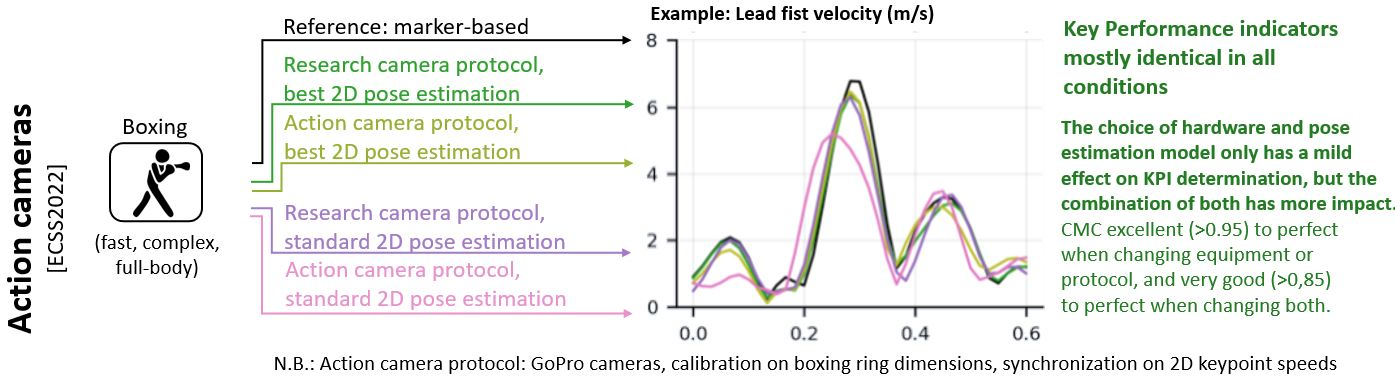
\includegraphics[width=\linewidth]{"../Intro/Figures/Fig_VisAbstract4.JPG"}
      \caption{Visual abstract for the assessment of KPIs in boxing with Pose2Sim \cite{Pagnon2022c}. \\Research camera protocol: Qualisys cameras, gold-standard calibration, hardware synchronization. Action camera protocol: GoPro cameras, calibration on boxing ring dimensions, synchronization on 2D keypoint speeds.}
	\label{fig_visabstract4}
\end{figure}


\newpage

\section{Introduction}

\subsection{Limits of research-grade systems in competitions}

When fine kinematic analysis is needed, the de facto approach is marker-based motion capture. However, we have seen that it is not appropriate in sports, and markerless methods are favored.

% since it involves gluing markers directly on the skin, which is not conceivable during a match or a training session. Markers are intrusive and cumbersome, and usually involve specific environmental conditions. Moreover, they can fall off the body when the athlete is sweating or moving fast. As a consequence, it is important to investigate markerless techniques. 

Moreover, competition conditions are often fast-paced and congested, and thus the capture system needs to be discrete and installed swiftly. As a consequence, research grade video systems such as Qualisys are not appropriate: they involve setting up large cameras and stands, with power and synchronization cables, which are obstructing and which prevent cameras from being spread too far apart. These systems require at least two trained operators to set them up and to adjust their parameters. They are also very expensive, while their framerate and resolution are not very good. 

On the other end, consumer-grade action cameras such as GoPros are very small, don't necessitate any cabling, and the operator has nothing to do but pressing the recording button. They are also cheap, and offer remarkably high framerate, resolution, and image quality. However, there is no centralized visual feedback upon recording, their battery does not last more than an hour, they don't come with calibration, and until recently, no simple synchronization solution existed. In any case, their use has been investigated lately. \cite{Jackson2016} tracked bees after calibrating with a wand and synchronizing on a sound signal, while \cite{Dalla2019} equipped cameras with an illumination ring and a subject with markers, and evaluated knee flexion after calibrating with a wand and synchronizing on a flashlight.

When outdoors, in direct sunlight and with large capture volumes, calibration of video cameras becomes delicate, too: markers on a calibration wand are inconstantly detected. No reliable solution currently exists, including with active LED markers. Checkerboard calibration is almost equally problematic, as corners are not always well detected unless the board is too large to conveniently carry around. Other solutions exist, such as calibrating intrinsic parameters with a checkerboard \cite{Zhang2000}, and extrinsic parameters with manually clicked and semi-automatically tracked points on a wand \cite{Argus,Jackson2016}. 
% Since there only 2 collinear points are tracked on a wand, extrinsic parameters cannot be calculated on one single frame. Hence, Argus assumes an \textit{a priori} calibration, triangulates wand points, and minimizes reprojection errors by sparse bundle adjustment (SBA) frame after frame, while being delivered additional wand points. Then 
% Essential matrix via 8 points algorithm, minimization via SVD (and not SBA?), decomposition of E to get projection matrice (and then homographic matrice by multiplying by K-1?)
Alternatively, it is possible to calibrate extrinsics on any object of known dimensions \cite{Dawson-Howe1994}, be it a human being \cite{Liu2022a}.

Lastly, synchronization can also be a problem. Using a trigger signal is the most accurate approach, but again, it generally involves using wired cameras. Other methods rely on using a flash, or an audio clap \cite{Jackson2016}, but they are not possible in the context of a competition. Moreover, as the sound does not travel instantaneously, the synchronization will not be very accurate on a large capture space if the distance from camera to sound source is not taken into account \cite{Hasler2009}. For example, a 20 meters difference would lead to a 60 ms shift, which represents 7 frames at 120 fps. Identifying the instant of a sharp movement is sometimes used as a time reference, but it is generally not accurate enough for a synchronization to the frame, especially if the framerate is high. Other procedures can be explored, such as WiFi synchronization \cite{Romanov2019} or Bluetooth synchronization \cite{Asgarian2022}, but they usually require using external devices. GPS synchronization is compatible with GoPro 9 and plus, but signal may not be available everywhere, typically in some sports halls \cite{GoPro2022}. Another way to synchronize data streams is to cross-correlate them, and to infer the delay between them from the time of maximum correlation \cite{Plotz2012}. 


\subsection{Key Performance Indicators in boxing}

Key Performance Indicators (KPIs) are a set of variables which need to be measured in priority, in order to assess performance, or to evaluate main areas where work is needed. Although they are more known in the fields of management or of the industry, identifying them is also important in sports \cite{Hughes2002,Butterworth2013}: they allow coaches to assess performance, and to tailor training to each athlete's specificities. Determining them would typically be done in two steps. First, through discussions with coaches, who usually have a subjective, but nevertheless very fine and comprehensive understanding of their sport. Then, the most relevant of these variables can be selected, for example by Principal Component Analysis (PCA) \cite{Hotelling1933}. PCA allows for grouping the variables that explain most of the performance, and excluding the others \cite{ODonoghue2008}.

However, this approach has the disadvantage that prior to pursuing any further statistical analysis, all the potential variables first need to be extensively recorded. Only then, the most relevant ones can be determined. Moreover, it might lead to the selection of indicators which can be hard to retrieve, or be not intuitively meaningful as they potentially consist in the linear combination of some seemingly unrelated variables. In this case, one can choose the performance indicator most associated with each principal component \cite{ODonoghue2008}. Other methods exist, such as exclusive expert coach opinion, hierarchical models obtained by breaking down individual techniques, or notational analysis based on scoring events and actions along a competition, or other inferential statistic methods such as regression analysis, and more \cite{Hughes2002,Butterworth2013}.

KPIs must be meaningful and specific to each sport discipline, and it should be possible to capture them in a context as close as possible to the competition one. Boxing is one of the disciplines involved in the PerfAnalytics project, and it covers a wide range of movements, which makes its study relevant. KPIs in boxing can be separated into several categories: action annotations (such as scored points, number of recorded jabs punches or dodges by leaning backwards \cite{Thomson2013}), anthropometric KPIs (such as arm length and muscle percentage \cite{Chaabene2015}), physiological (such as velocity at maximal oxygen uptake and anaerobic power \cite{Chaabene2015}), or biomechanical (such as ground reaction force of the rear leg before execution of a cross punch, activation of the latissiums dorsi during the hook punch, or extension of the elbow at the end of the execution of the jab \cite{Lenetsky2020}). 

Among all these KPIs, we focus on a subset of the biomechanic ones, namely kinematics. Ultimately, a decisive aspect in a punch is its speed. First, a fast punch is difficult for the opponent to dodge. Then, speed multiplied by force is equal to punch power. In addition, punch force is also correlated to hand velocity \cite{Mack2010}. However, speed is not generated the same way in jabs as in hooks, since one is a mostly translational movement whereas the other is mostly rotational. \cite{Lenetsky2020} broke down the phases of both techniques. Among other body motions, the jab first involves translating the lead foot toward the target, then the pelvis and the torso, while the lead arm flexes at the elbow to store elastic energy prior to throwing the punch. Finally, the elbow extends, until the fist is brought into contact with the target. Regarding the rear hook, it starts with flexing the rear knee, while the pelvis and torso rotate horizontally away from the target. Then the motion is reversed, as the knee extends and the pelvis and torso rotate toward the target. Lastly, the attacking arm abducts at the shoulder until the fist reaches the target. 

As a consequence, it appears that lead foot translation, pelvis translation, lead elbow extension, and lead fist velocity would consist in good KPI variables for the jab. Similarly, rear knee flexion, pelvis rotation, rear shoulder extension, and rear fist velocity would be valuable to characterize the rear hook. 


\subsection{Objectives}

Evaluating kinematic KPIs in boxing is inconvenient with marker-based techniques, and challenging with markerless ones. Indeed, boxing movements are fast, 3 dimensional, and involve the whole body. Moreover, addressing motion capture in an ecologically valid context involves dealing with constraints on the protocol, and requires carefully thinking about the hardware, the calibration method, and the synchronization procedure. These three elements determine 3D reconstruction. However, before this stage comes the 2D pose estimation. 

Numerous solutions exist in this regard. AlphaPose \cite{Fang2017} and OpenPose \cite{Cao2019} are both the most common and the most accurate \cite{Needham2021b,Mroz2021}. OpenPose is even more widely used than AlphaPose, hence this is the one we choose to focus on. Its standard model is body\_25, however the body\_25B subset of the single-network whole-body pose estimation \cite{Hidalgo2019} also provides 25 points, is as fast as the standard one, and is claimed to be more accurate and to reduce false positives \cite{Hidalgo2019,Pagnon2021}. 

The objective of this study is to evaluate how accurately KPIs can be retrieved in real-life sports conditions, concurrently with a marker-based analysis. Results will be evaluated for a research-grade markerless system, for a consumer-grade markerless one with post-calibration and post-synchronization, as well as with a slightly less accurate pose estimation model in both previous conditions. A subsidiary question is whether the 3D reconstruction procedure has more or less impact on accuracy than the choice of a 2D pose estimation model.


\section{Methods}
\subsection{Participants and protocol}
3 adult elite boxers were selected, from different weight categories and with different morphologies: one right-handed female, one right-handed male, and one left-handed male. Details are provided in Table~\ref{table:participants_details}. They all provided informed written consent. Participants were equipped with 44 reflective markers, placed by one single operator, following the recommendations of the International Society of Biomechanics (ISB) \cite{Wu2002, Wu2005}. Marker set and marker placement are detailed Figure~\ref{fig_mkboxe}.

A professional coach instructed the athletes to perform a sequence of shadow-boxing 6 times, consisting in a jab, a high rear hook, and a low rear hook. They executed these movements in their usual training center, on a competition boxing ring. 

\begin{table}[!ht]
      \centering
      \begin{tabular}{llllll}
          \toprule
          \textbf{Participant} & \textbf{Gender} & \textbf{Handedness} & \textbf{Age (years)} & \textbf{Height (m)} & \textbf{Weight (kg)} \\ 
          \specialrule{0.14 em}{0pc}{0pc}
          1 & Male & Right-handed & 20 & 1.72 & 54 \\ 
          2 & Female & Right-handed & 19 & 1.63 & 59\\ 
          3 & Male & Left-handed & 18 & 1.90 & 78\\ 
          \bottomrule
      \end{tabular}
      \caption{Demographic details on the participants.}
        \label{table:participants_details}
\end{table}

\begin{figure}[!ht]
	\centering
	\def\svgwidth{1\columnwidth} 
	\fontsize{10pt}{10pt}\selectfont
	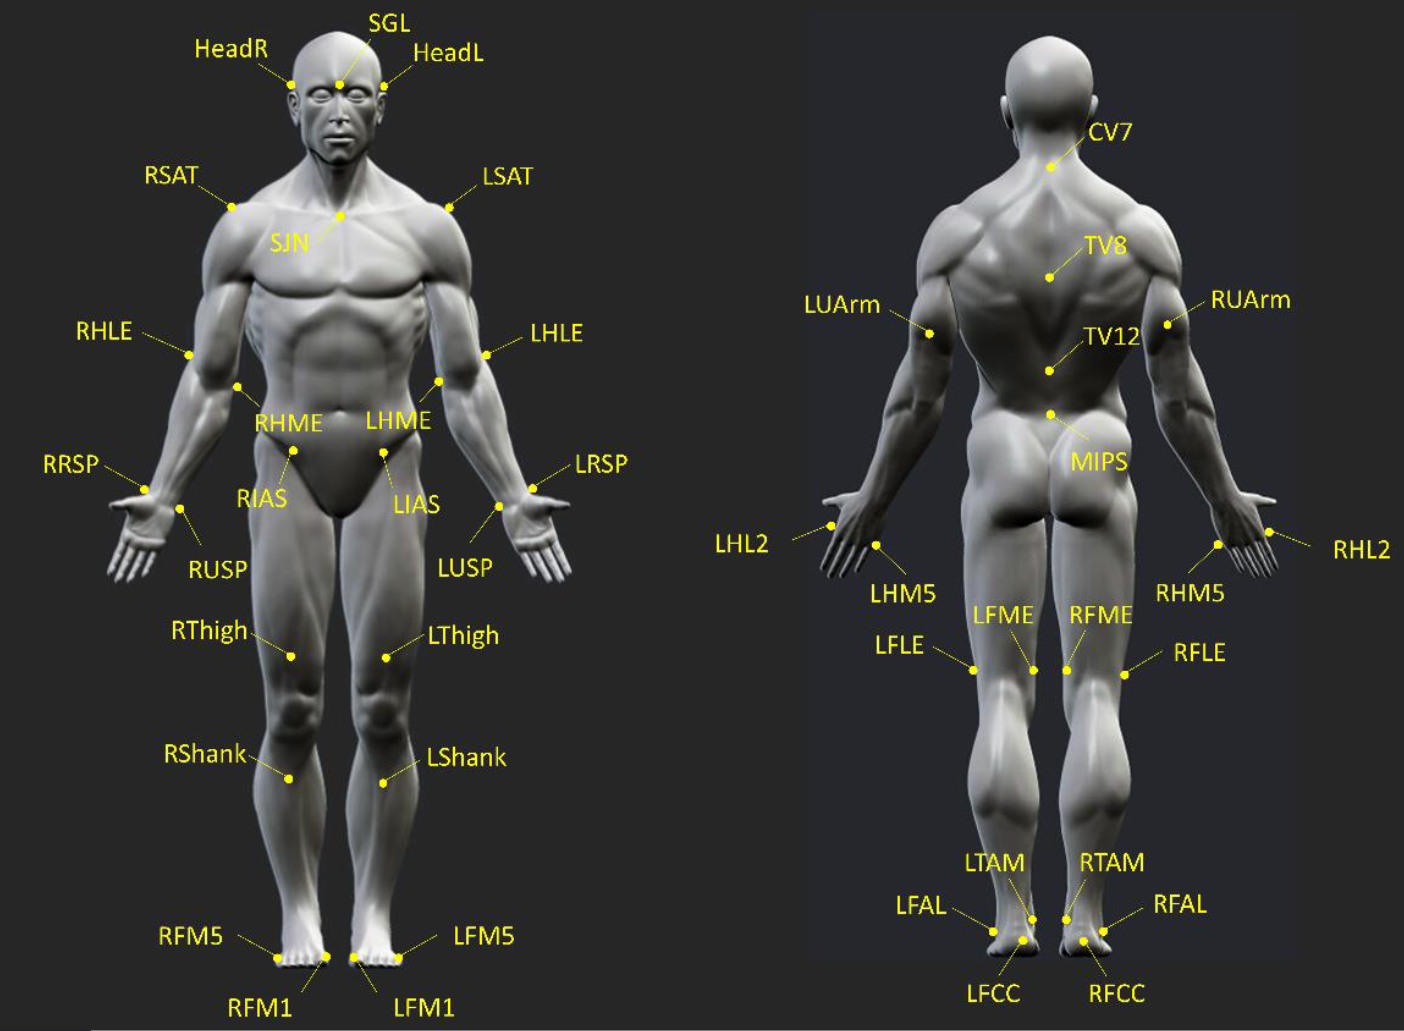
\includegraphics[width=\linewidth]{"../Chap6/Figures/Fig_MkBoxe.PNG"}
	\caption{Marker location on the body \cite{Lahkar2022b}.}
	\label{fig_mkboxe}
\end{figure}

The boxing sequences were recorded by 12 opto-electronic Qualisys cameras (7 Miqus M3, resolution 2 MP, framerate 300 fps; and 5 Arqus A5, resolution 5 MP, framerate 300 fps), 8 video Qualisys cameras (Miqus videos, resolution 2 MP, framerate 60 fps), and 8 GoPros (4 GoPro 7 and 4 GoPro 8, 2 MP, 120 fps, linear field of view). GoPro videos were down-sampled to 60 fps before pursuing further analysis. Marker-based and markerless Qualisys cameras were placed next to each other as pairs, except for the 2 surplus optoelectronic cameras. Aperture, focus, shutter speed, and other parameters were carefully adjusted by hand. Both data streams were recorded within the Qualsys QTM software, which allowed for calibration and synchronization, and for a common frame of reference. GoPro cameras did not need any adjustment prior to recording. However, calibration and synchronization were performed after the capture, following the methods proposed in the next two sections. 

Marker-based 3D coordinates were calculated with the Qualisys QTM software. These marker data were augmented with joint center coordinates: shoulder centers were defined based on the regression equations adopted from \cite{Dumas2018}, and elbow, wrist, knee, and ankle joints were defined as the midpoints between epicondyle markers \cite{Pohl2010}. Markerless videos from GoPro and Qualisys cameras were processed by OpenPose v1.6 \cite{Cao2019}, both with body\_25 and body\_25B models. Once calibration and camera synchronization were solved (see next two sections), tracking, triangulation, and filtering were done with Pose2Sim \cite{Pagnon2022b}. Both marker-based and markerless 3D coordinates were processed by a 10 Hz, 4th order low-pass Butterworth filter \cite{Butterworth1930}, which was deemed appropriate to filter out noise without missing peak values. Inverse kinematics of both were processed with the same OpenSim model \cite{Pagnon2022b}, in order to not interfere with the other protocol variations which were actually investigated.


\subsection{Post-calibration on ring dimensions}\label{calib_pnp}

Unlike with Qualisys optoelectronic and video cameras, there is no live calibration procedure for GoPros. Intrinsic parameters were computed priorly by filming a checkerboard of known dimensions from different distances and orientations. Corners were found, and their locations were refined with OpenCV \cite{Bradski2000}. This allowed for focal length, optical center, and distortion parameters to be calculated \cite{Zhang2000}. See Table~\ref{table:tab_intrinsic} for a summary of the GoPro 7 and 8 intrinsic parameters.

\begin{table}[!ht]
    \centering
    \resizebox{0.85\textwidth}{!}{
    \begin{tabular}{lllll}
        \toprule
        \textbf{Model} & \textbf{Field of view} &\textbf{Resolution (px)} & \textbf{Focal length (px)} & \textbf{Distortion coefficients}\\ 
        \specialrule{0.14 em}{0pc}{0pc}
        GoPro 7 & Linear & 1920x1080 & 1029 & [-0.004, 0.004, 0.0] \\ 
        GoPro 8 & Linear & 1920x1080 & 915 & [-0.01, 0.004, -0.0015]\\ 
        \bottomrule
    \end{tabular}}
    \caption{Intrinsic parameters of the GoPro 7 and GoPro 8 cameras. The optical center was assumed to be at the center of the image. Focal length was supposed to be identical in both directions, the pixel to be square and not skewed, and $6^{th}$ order radial and $2^{nd}$ order tangential distortion coefficient to be null.}
      \label{table:tab_intrinsic}
\end{table}

\newpage
Extrinsic parameters can then be solved by pairing global 3D coordinates of an object to its corresponding 2D coordinates on the image. This is classically done with a frame or a checkerboard laid on the floor (where it can be seen by all cameras), but when cameras are too low or too far from the center of the scene, image coordinates can be imprecise and lead to inaccurate extrinsic calibration. In this case, any object of known dimensions on the scene can be used: in our case, we measured the ring dimensions, and retrieved the corresponding 2D coordinates on each camera view. We then used the Perspective-n-Point (PnP) algorithm using non-linear Levenberg-Marquardt minimization scheme \cite{More1978} to solve extrinsic parameters \cite{Marchand2015} (see Figure~\ref{fig_calib}). Dimensions of the ring were measured approximately, thus we iteratively adjusted its coordinates in order to minimize the grand average error for all cameras between 2D coordinates and projected 3D coordinates, until all camera errors stayed under 3 cm. 

\begin{figure}[!ht]
	\centering
	\def\svgwidth{1\columnwidth}
	\fontsize{10pt}{10pt}\selectfont
	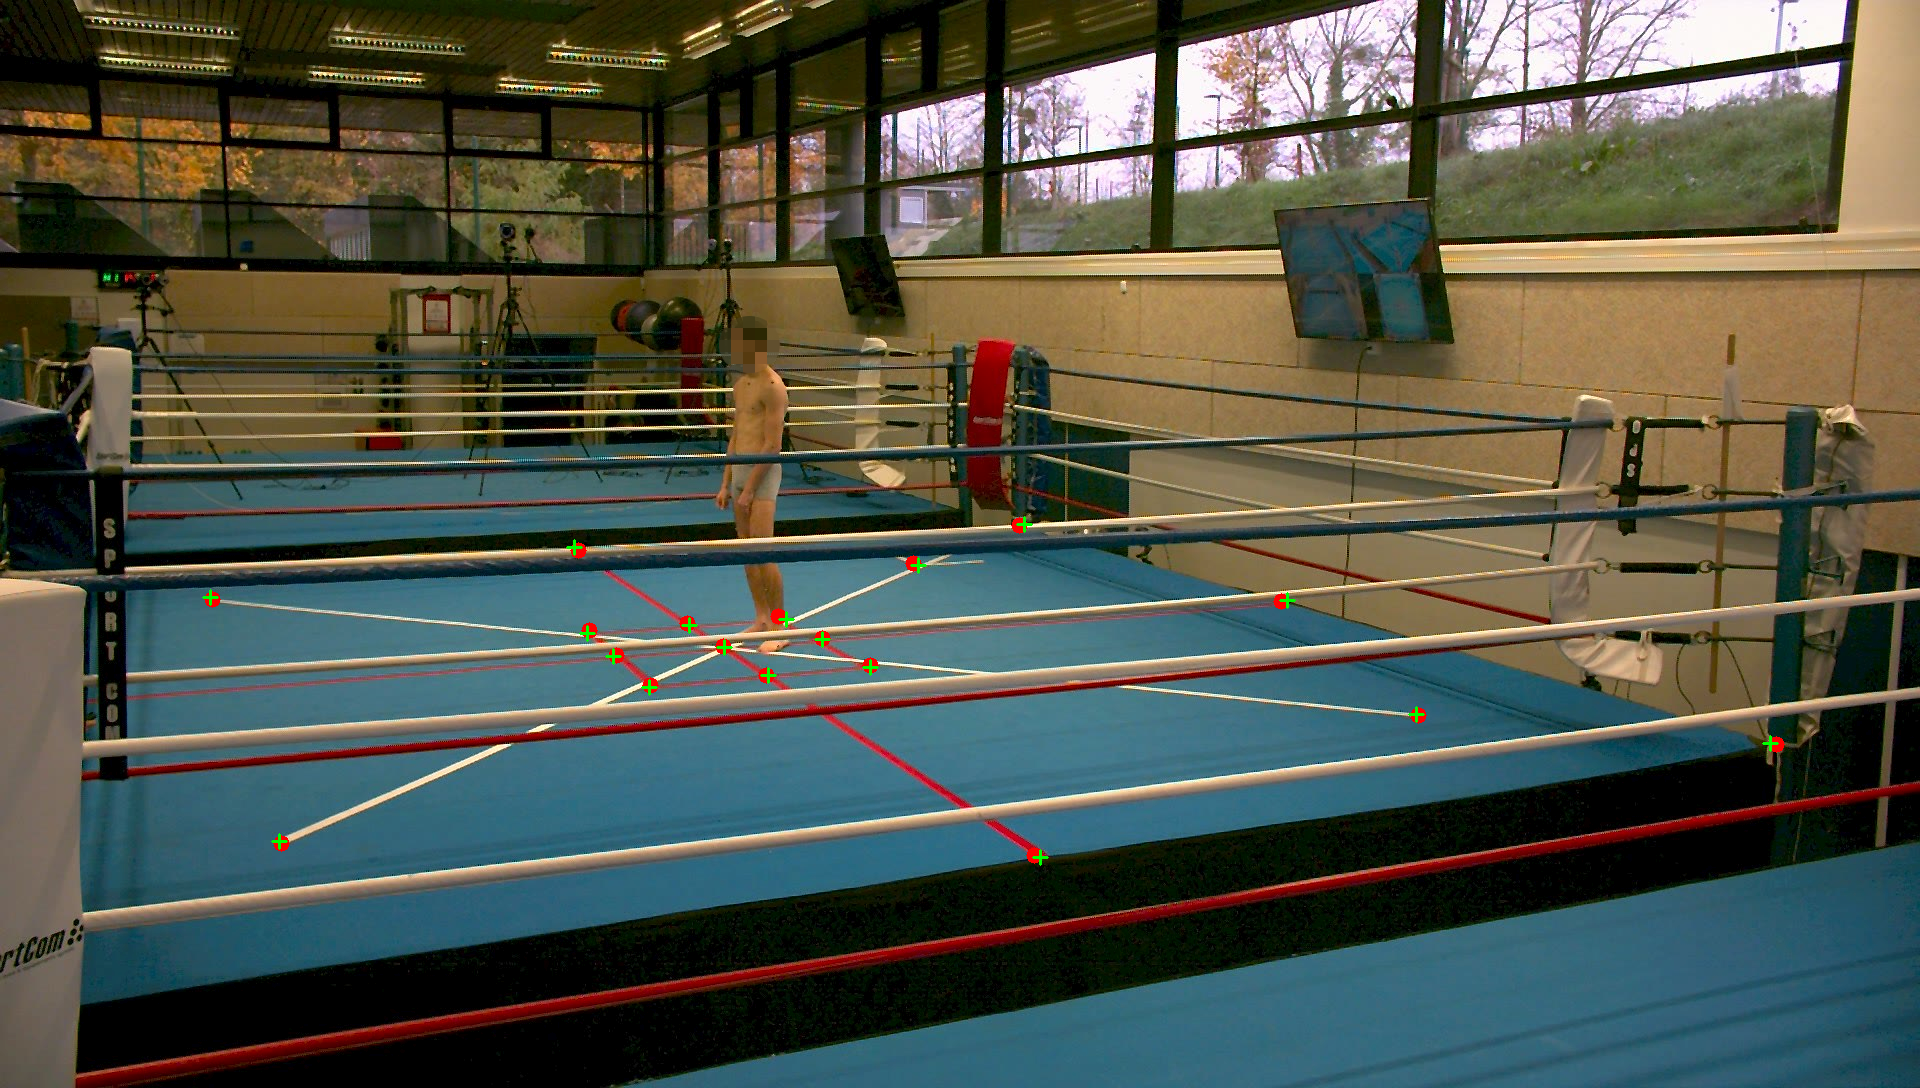
\includegraphics[width=\linewidth]{"../Chap6/Figures/Fig_Calib.png"}
	\caption{Extrinsic calibration on ring dimensions. Green crosses represent the 2D points of the ring clicked by the user, and red dots its 3D coordinates projected on the image plane.}
	\label{fig_calib}
\end{figure}


\subsection{Post-synchronization on 2D movement speeds}

GoPro videos were roughly cut to select the approximate same sequence from all cameras. OpenPose 2D keypoint trajectories were differentiated, in order to obtain 2D keypoint speeds. We assumed that two nearby cameras were synchronized when 2D speeds were maximally correlated. This is the approach adopted independently explored by OpenCap \cite{Uhlrich2022}.

Hence, we used time-lagged cross-correlation to determine this offset (Figure~\ref{fig_sync}). This can be done for one specific point, or for all of them at once with attributing a different weight to each keypoint. Typically, larger weights could be attributed to fists or to other fast moving keypoints. In practice, all weights were set to 1, since it made results more robust without causing them to be less accurate.

\begin{figure}[!ht]
	\centering
	\def\svgwidth{1\columnwidth}
	\fontsize{10pt}{10pt}\selectfont
	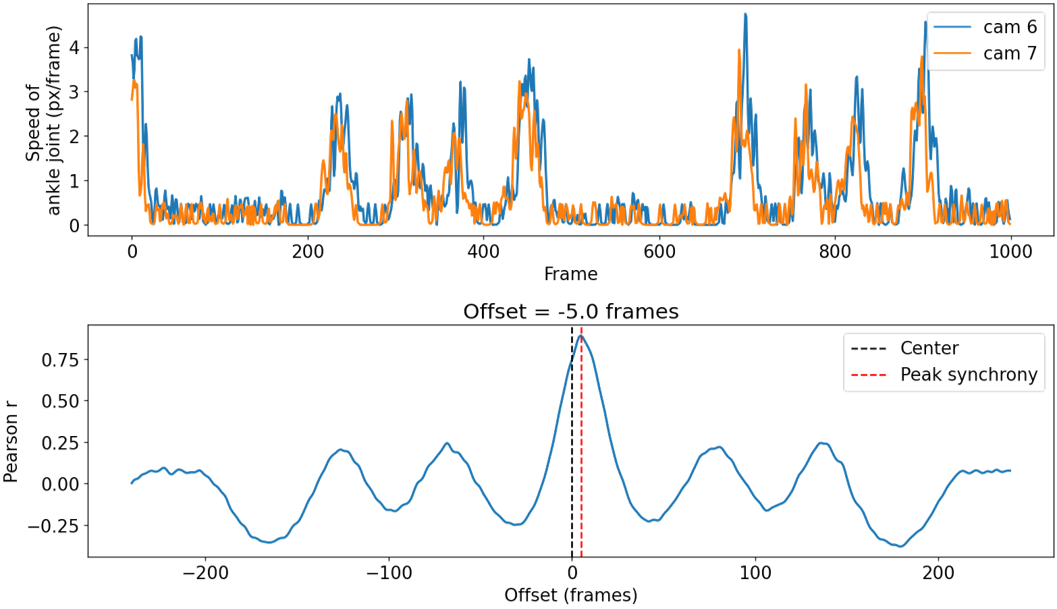
\includegraphics[width=\linewidth]{"../Chap6/Figures/Fig_Sync.png"}
	\caption{\textit{Top:} 2D keypoint speed comparison between two cameras. \textit{Bottom:} The offset frame with maximum correlation corresponds to the synchronization offset.}
      \label{fig_sync}
\end{figure}


\FloatBarrier
\subsection{GoPro to Qualisys spatio-temporal coordinate system}

In order to be able to compare GoPro results to Qualisys ones, they need to share a common spatio-temporal base. We synchronized both 3D coordinates outputs in the same way as previously described, however with 3D instead of 2D speeds. Then, we transformed GoPro 3D coordinate results to the Qualisys' coordinate system. The rotation and translation needed were found by minimizing the differenc between GoPro and Qualisys 3D coordinates.


\subsection{Statistical analysis}

Calibration accuracy was assessed by comparing residual reprojection errors with the GoPro protocol to those with the Qualisys one. There is no objective metric for assessing synchronization accuracy, however we estimated it indirectly. Once GoPro cameras were synchronized two by two, we retrieved the resulting Pearson correlation coefficient between 2D speeds, and averaged it across all cameras. Similarly, we calculated the same coefficient for the perfectly synchronized Qualisys system. Assuming that GoPro cameras are approximately spread out in the same way as Qualisys ones, and that the 2D pose estimation performed similarly well in both cases, any correlation difference would probably be due to the non-perfect post-synchronization of GoPro cameras. A correlation is generally considered to be weak if r<0.5, moderate if 0.5<r<0.7, and strong if r>0.7.

We examined time series for lead foot translation, pelvis translation, lead elbow extension, and lead fist velocity for the jab; and rear knee flexion, pelvis rotation, rear shoulder extension, and rear fist velocity for the rear hook. 
% Different technique (high inter-participant variability), but reproducible (low intra-participant variability). Inter-protocol variability almost non existent.
Waveform similarity between the reference marker-based method and all other markerless ones was assessed with the inter-protocol coefficient of multiple correlation (CMC) \cite{Ferrari2010}, which quantifies in one single value the concurrent effects of differences in correlation, gain, and offset (see \nameref{stats_accuracy} \autoref{ch:5}). We compared the Root Mean Square Error (RMSE) with marker-based results to the findings of two previous studies done with the commercial markerless software Theia3D \cite{Kanko2021b}.

\newpage
We also retrieved certain quantifiable indicators on the aforementioned recorded variables. Ranges of motion and onset times were examined for translations, and peak values and times for angles and speeds. 
% Onset time: threshold (depending on variables and on subject) on moving average over 3 frames (0.05 s)
We computed mean differences and standard deviation (std) between marker-based results and all other protocol results. The impact of the camera type, and of the 2D pose estimation model, were similarly explored. 

Normality of the distribution of differences was verified with a Shapiro-Wilk test \cite{Shapiro1965}. If this condition was satisfied, we used paired t-tests to test the null hypothesis that there was no statistical difference between protocols \cite{Student1908}. If not, we used the Wilcoxon signed-rank test \cite{Wilcoxon1945}. When some paired differences were equal to zero, the normal approximation was used. When less than 10 of the paired differences were non-zero, we could not reject the null hypothesis that mean paired results were equal. We used a significance level of 0.05.


\section{Results}

\subsection{Calibration and synchronization accuracies}

Calibrating GoPro cameras on ring dimensions led to an average of 2.59 px reprojection error, which corresponds to 1.93 cm of error at the center of the scene. Conversely, Qualisys average residuals for calibration stayed under 1 mm, which is approximately 20 times better. After synchronization, Pearson correlation coefficient between 2D speeds was 0.69 in average (moderate correlation) with the GoPro system, while it was 0.73 in average (strong correlation) with the Qualisys one, which denotes a non-perfect synchronization of the GoPro cameras. 


\subsection{Waveform comparison}

Waveforms were very dissimilar across participants, especially for the hook technique. For example, no apparent peak could be found on hook trials for subject 2 on rear knee flexion nor on rear shoulder abduction. On the opposite, differences were almost imperceptible across protocols (Figure~\ref{fig_graphkpi}). Results of the research-grade markerless setup, with specialized cameras, marker-based calibration, and hardware synchronization, were almost identical to those of the marker-based analysis (CMC > 0.99). Results from GoPro cameras with calibration on ring dimensions and synchronization on 2D keypoint speeds were also in excellent agreement (CMC > 0.95). The same was true with Qualisys cameras used with the default body\_25 model (CMC > 0.95). However, the combined use of GoPro cameras and of the default body\_25 OpenPose model led to a slight decrease in accuracy, even if results were still in very good agreement (CMC > 0.85). Velocities and shoulder rotation were the least in agreement, although CMC stayed over 0.90 (Table~\ref{table:tab_cmcboxe}).

More precisely, in the most favorable conditions, the RMSEs amounted to 8.5 mm for lead foot translation (which can be compared to 24 mm for ankle translation during gait for Theia3D \cite{Kanko2021b}), 7.9 mm for pelvis translation (vs. 36 mm for hip translation), 4.1° for lead elbow extension (vs. 7.4° for Theia3D in the same boxing settings \cite{Lahkar2022b}), 0.3 m/s for lead and rear fist velocities (vs. 0.1° and 0.2 m/s \cite{Lahkar2022b}), 3.2° for knee flexion (vs. 3.3° \cite{Kanko2021b}), 6.5° for pelvis rotation (vs. 8.5° \cite{Kanko2021b}), 6.5° for shoulder abduction (vs. 6.3° \cite{Lahkar2022b}). Results were slightly degraded when using GoPro cameras \emph{or} the standard body\_25 model, but they still remained comparable to the Theia3D results. When using both GoPro cameras \emph{and} the body\_25 model, they became more clearly worse, except for translations for which errors remained comparable (Table~\ref{table:tab_cmcboxe}).

\begin{figure}[!ht]
	\centering
	\def\svgwidth{1\columnwidth}
	\fontsize{10pt}{10pt}\selectfont
	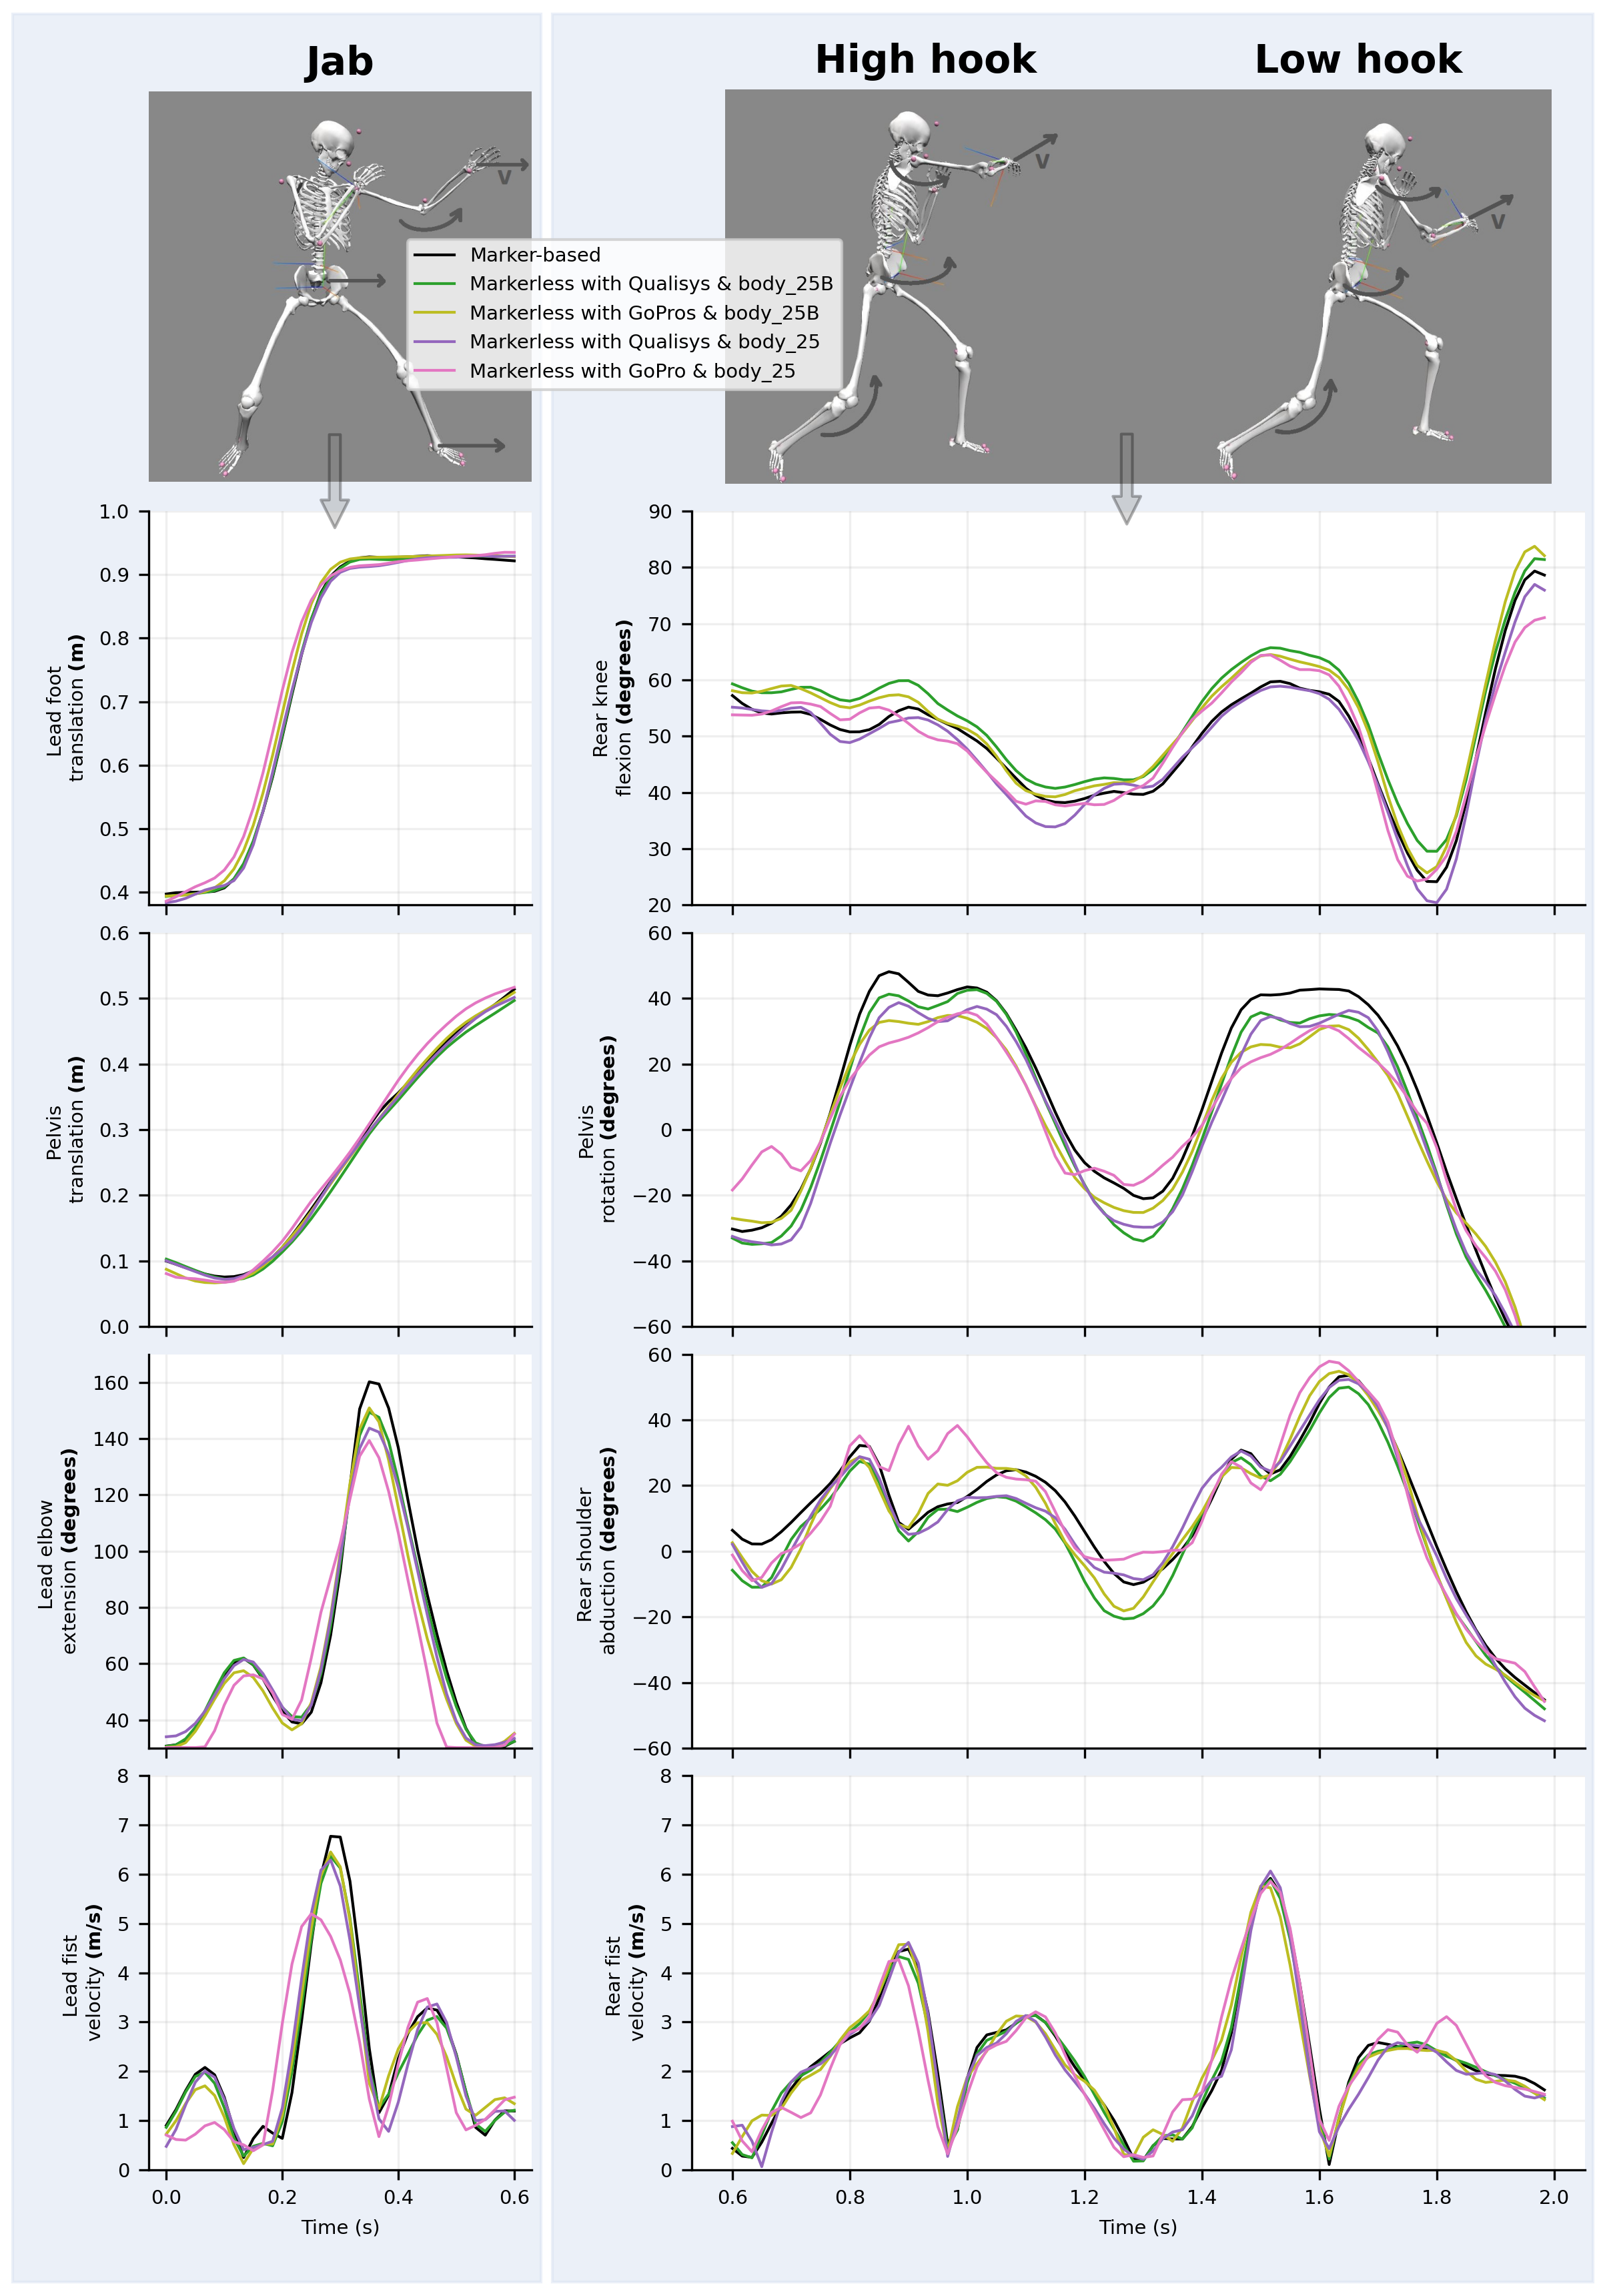
\includegraphics[width=1\linewidth]{"../Chap6/Figures/Fig_GraphKPI.png"}
	\caption{A representative trial by one of the athletes. Comparison of selected variables for a sequence of jab, high hook, and low hook in boxing. Waveforms look very similar across all protocols, even though the use of the standard OpenPose body\_25 model instead of the experimental body\_25B one seems to cause more discrepancy when compared to the reference marker-based analysis.}
	\label{fig_graphkpi}
\end{figure}

\FloatBarrier
\begin{table}[!ht]
      \centering
      \resizebox{\textwidth}{!}{
      \begin{tabular}{lllll}
          \toprule
          \shortstack{\\ \textbf{Marker-based vs. $\rightarrow$}} & \shortstack{\textbf{Markerless}\\\textbf{with Qualisys}} & \shortstack{\textbf{Markerless}\\ \textbf{with GoPros}} & \shortstack{\textbf{Markerless with}\\\textbf{Qualisys \& body\_25}} & \shortstack{\textbf{Markerless with}\\\textbf{GoPros \& body\_25}} \\
          \midrule
          \textbf{CMC} & \multicolumn{4}{c}{Jab punch} \\
          \cmidrule(l{2pt}r{2pt}){2-5}
          Lead foot translation & 1.00 & 1.00 & 1.00 & 1.00\\
          Pelvis translation & 1.00 & 1.00 & 1.00 & 1.00\\
          Lead elbow extension & 1.00 & 0.98 & 0.99 & 0.95\\
          Lead fist velocity & 0.99 & 0.97 & 0.98 & 0.91\\
          \cmidrule(l{2pt}r{2pt}){2-5}
          ~ & \multicolumn{4}{c}{Hook punches} \\
          \cmidrule(l{2pt}r{2pt}){2-5}
          Rear knee flexion & 0.99 & 0.99 & 0.99 & 0.99\\
          Pelvis rotation & 0.99 & 0.99 & 0.99 & 0.98\\
          Rear shoulder rot. & 0.99 & 0.99 & 0.99 & 0.95\\
          Rear fist velocity & 0.99 & 0.97 & 0.98 & 0.90\\
                              \midrule
          \textbf{RMSE} & \multicolumn{4}{c}{Jab punch} \\
          \cmidrule(l{2pt}r{2pt}){2-5}
          Lead foot translation (mm) & 8.5 & 20.5 & 9.5 & 34.6\\
          Pelvis translation (mm) & 7.9 & 8.3 & 8.3 & 15.6\\
          Lead elbow extension (°) & 4.1 & 10.3 & 6.2 & 17.4\\
          Lead fist velocity (m/s) & 0.3 & 0.5 & 0.5 & 0.9\\
          \cmidrule(l{2pt}r{2pt}){2-5}
          ~ & \multicolumn{4}{c}{Hook punches} \\
          \cmidrule(l{2pt}r{2pt}){2-5}
          Rear knee flexion (°) & 3.2 & 4.1 & 3.2 & 3.9\\
          Pelvis rotation (°) & 6.9 & 8.6 & 8.1 & 11.4\\
          Rear shoulder rotation (°) & 6.5 & 8.0 & 7.3 & 14.2 \\
          Rear fist velocity (m/s) & 0.3 & 0.5 & 0.4 & 0.9\\
          \bottomrule
      \end{tabular}}
      \caption{The Coefficient of Multiple Correlation (CMC) was used to assess the waveform similarity of the variables of interest. Agreement is deemed excellent if CMC>0.95, and very good if CMC>0.85 \cite{Ferrari2010}. Root Mean Square Errors (RMSEs) were also reported.}
      \label{table:tab_cmcboxe}
\end{table}


\subsection{KPI accuracy assessment}

As KPI differences across protocols were never normally distributed, paired t-tests could not be rigorously performed. As a consequence, we only used Wilcoxon signed-rank tests. Nonetheless, in many cases, especially for time results, most paired differences were equal to zero. In these instances, we could not reject the null hypothesis that results were identical in average. It should be noted that for rear knee flexion and for rear shoulder abduction in hook punches, KPI means and standard deviations did not take participant 2 into account, since her movement patterns did not present any peak in these variables.
% In any case, no clear conclusion could be drawn from tests of significance. KPI results were more often significantly different from marker-based ones for magnitudes than for times, and for jabs than for hooks, regardless of the protocol (Table~\ref{table:tab_peakboxe}). The same can be said of the significance of differences across camera types, and across 2D pose estimation models (Table~\ref{table:tab_protoc}).

Range of motion errors usually remained under $\approx$10 mm, as compared to the marker-based protocol. Mean errors were even lesser with body\_25 model, but with more variation around the mean, which did not lead to any significant differences. Elbow extension, knee extension (calculated as \textit{180° $-$ knee flexion}), shoulder abduction, and pelvis rotation peak angles were generally underestimated, by 2.9° to 5.4° with the Qualisys cameras and body\_25B model, by 2.7° to 10.2° when using GoPro cameras or body\_25 model, and by more than 11.8° to 17.2° when using the most suboptimal protocol with both GoPro cameras and body\_25 model. Peak fist velocity errors did not broadly depend on the choice of protocol. However, they were underestimated by up to 0.4 m/s (1.4 km/h) for both hands (Table~\ref{table:tab_peakboxe}).

Peak times were usually estimated too early with GoPro cameras, by about 10 to 40 ms, i.e., 0.6 to 2.4 frames at 60 fps. Most other onset and peak time errors were not statistically significant, especially for Qualisys cameras when used with the experimental Body\_25B pose estimation model. Rear shoulder abduction demonstrated the largest peak time error, up to about 50 ms (3 frames) (Table~\ref{table:tab_peakboxe}).

\begin{table}[!ht]
      \centering
      \resizebox{\textwidth}{!}{
      \begin{tabular}{lcccc}
          \toprule
          \shortstack{\textbf{\(\mathbf{Mean_{err}}\) ($\pm$std) of }\\ \textbf{Marker-based vs. $\rightarrow$}} & \shortstack{\textbf{Markerless}\\\textbf{with Qualisys}} & \shortstack{\textbf{Markerless}\\ \textbf{with GoPros}} & \shortstack{\textbf{Markerless with}\\\textbf{Qualisys \& body\_25}} & \shortstack{\textbf{Markerless with}\\\textbf{GoPros \& body\_25}} \\
          \midrule
          \textbf{ROM\(^1\) \emph{or} Peak value} & \multicolumn{4}{c}{Jab punch} \\
          \cmidrule(l{2pt}r{2pt}){2-5}
          \raggedleft Lead foot translation\(^1\) (mm) & -10.6 ($\pm$6.7) * & -10.0 ($\pm$7.4) * & -1.1 ($\pm$9.8) & 4.9 ($\pm$12.0) \\
          \raggedleft{Pelvis translation\(^1\) (mm)} & -6.9 ($\pm$6.0) * & 4.3 ($\pm$5.3) * & -4.1 ($\pm$7.4) & 11.2 ($\pm$9.5) * \\
          Lead elbow extension (°) & -2.9 ($\pm$2.0) & -8.6 ($\pm$3.5) * & -10.2 ($\pm$4.3) * & -17.2 ($\pm$6.1) * \\
          Lead fist velocity (m/s) & -0.4 ($\pm$0.1) * & -0.2 ($\pm$0.2) * & -0.4 ($\pm$0.2) * & -0.4 ($\pm$0.2) * \\
          \cmidrule(l{2pt}r{2pt}){2-5}
          ~ & \multicolumn{4}{c}{Hook punches} \\
          \cmidrule(l{2pt}r{2pt}){2-5}
          Rear knee flexion\(^2\) (°) & 5.4 ($\pm$1.9) * & 4.0 ($\pm$2.1) * & -0.5 ($\pm$1.9) & 1.7 ($\pm$2.8) \\
          Pelvis rotation (°) & -3.9 ($\pm$4.8) * & -7.9 ($\pm$2.7) * & -6.9 ($\pm$4.1) * & 11.8 ($\pm$5.7) *\\
          Rear shoulder abduction\(^2\) (°) & -4.1 ($\pm$2.2) * & -2.7 ($\pm$2.9) & -3.4 ($\pm$2.7) * & -0.9 ($\pm$6.2) \\
          Rear fist velocity (m/s) & -0.1 ($\pm$0.1) * & -0.4 ($\pm$0.2) & -0.3 ($\pm$0.1) * & -0.4 ($\pm$0.6) \\
          \midrule
          \textbf{Onset time\(^1\) \emph{or} Peak time} & \multicolumn{4}{c}{Jab punch} \\
          \cmidrule(l{2pt}r{2pt}){2-5}
          Lead foot translation\(^1\) (ms) & -0.9 ($\pm$2.3) & -14.8 ($\pm$11.4) * & -1.9 ($\pm$5.3) & -34.3 ($\pm$18.2) * \\
          Pelvis translation\(^1\) (ms) & 6.5 ($\pm$8.7) & -7.4 ($\pm$13.8) & 7.4 ($\pm$5.3) * & -14.8 ($\pm$18.2) * \\
          Lead elbow extension (ms) & -3.7 ($\pm$5.3) & -2.8 ($\pm$11.9) & -3.7 ($\pm$6.4) & -19.4 ($\pm$19.8) * \\
          Lead fist velocity (ms)& -8.3 ($\pm$8.8) & -13.0 ($\pm$9.8) * & -10.2 ($\pm$10.4) * & -20.4 ($\pm$15.1) * \\
          \cmidrule(l{2pt}r{2pt}){2-5}
          ~ & \multicolumn{4}{c}{Hook punches} \\
          \cmidrule(l{2pt}r{2pt}){2-5}
          Rear knee flexion\(^2\) (ms) & 15.3 ($\pm$27.0) & 9.7 ($\pm$31.2) & -19.4 ($\pm$34.5) & -19.4 ($\pm$48.2) \\
          Pelvis rotation (ms) & 18.5 ($\pm$41.8) & 28.5 ($\pm$49.5) & 31.5 ($\pm$58.0) * & 32.4 ($\pm$38.2) * \\
          Rear shoulder abduction\(^2\) (ms) & -58.3 ($\pm$52.1) & -40.3 ($\pm$45.0) * & -56.4 ($\pm$59.6) & -15.3 ($\pm$55.5) \\
          Rear fist velocity (ms) & 0.9 ($\pm$2.3) & -7.4 ($\pm$19.4) * & -2.8 ($\pm$9.0) & -14.8 ($\pm$28.0) * \\
          \bottomrule
      \end{tabular}}
      \caption{Mean and standard deviation ($\pm$std) errors of the boxing KPIs captured through each protocol, as compared to marker-based reference results. \(^1\)Peak values and times were observed for rotations and speeds, and ROMs and onset times for translations. \(^2\)Participant 2 was not taken into account in rear knee flexion nor on rear shoulder abduction results, since her movement patterns did not lead to any peak in these variables.  ROM: Range Of Motion. *indicates statistically significant differences (p<0.05).}
      \label{table:tab_peakboxe}
\end{table}


Using GoPros instead of Qualisys cameras had a comparable impact as switching back to the standard body\_25 OpenPose model on ranges of motion (up to 13 mm difference), peak angles (up to 7°), and peak velocities (0.1 m/s). However, using GoPro cameras lead to larger delays than choosing the body\_25 model: about 20 ms vs. 10 ms (1.2 vs; 0.6 frames) for translations, and 10 ms vs. 5 ms (0.6 vs. 0.3 frames) for velocities. No general conclusion could be drawn for time differences in joint angles, as peaks were more challenging to accurately detect, especially when using the body\_25 model which led to noisier waveforms (Table~\ref{table:tab_protoc}).

\begin{table}[!ht]
      \centering
      \resizebox{\textwidth}{!}{
      \begin{tabular}{lcccc}
            \toprule
            ~ & \multicolumn{2}{c}{\textbf{Qualisys vs. GoPros}} & \multicolumn{2}{c}{\textbf{Body\_25B vs. Body\_25}}\\
            \cmidrule(l{2pt}r{2pt}){2-3} \cmidrule(l{2pt}r{2pt}){4-5}
            \shortstack{\(\mathbf{Mean_{err}}\) \textbf{($\pm$std)} \\~} & \shortstack{\textbf{ROM\(^1\) \emph{or} Peak value}\\(mm, °, or m/s)} & \shortstack{\textbf{Onset\(^1\) \emph{or} Peak time}\\(ms)} & \shortstack{\textbf{ROM\(^1\) \emph{or} Peak value} \\(mm, °, or m/s)} & \shortstack{\textbf{Onset\(^1\) \emph{or} Peak time}\\(ms)} \\
            \cmidrule(l{2pt}r{2pt}){2-2} \cmidrule(l{2pt}r{2pt}){3-3}
            \cmidrule(l{2pt}r{2pt}){4-4} \cmidrule(l{2pt}r{2pt}){5-5}
            \textbf{Jab}\\
            Lead foot translation\(^1\) & 3.3 ($\pm$8.9) * & -23.1 ($\pm$18.9) * & 12.2 ($\pm$10.9) * & -10.2 ($\pm$16.1) *\\
            Pelvis translation\(^1\) & 13.3 ($\pm$10.4) * & -18.1 ($\pm$18.4) * & 4.8 ($\pm$8.2) * &-3.2 ($\pm$15.8) \\
            Lead elbow extension & -6.5 ($\pm$10.8) * & -7.4 ($\pm$16.6) * & -7.8 ($\pm$9.5) * & -8.3 ($\pm$17.1) *\\
            Lead fist velocity & 0.1 ($\pm$0.2) * & -7.4 ($\pm$15.7)  & -0.1 ($\pm$0.2) * & -4.6 ($\pm$11.0) *\\
            \\
            \textbf{Hook}\\
            Rear knee flexion\(^2\) & 0.5 ($\pm$3.2) & -2.8 ($\pm$29.8) & -4.1 ($\pm$2.6) * & -31.9 ($\pm$58.8) * \\
            Pelvis rotation &  -4.4 ($\pm$6.9) * & 5.5 ($\pm$59.8) * & -3.5 ($\pm$5.2) & 8.4 ($\pm$50.7)\\
            Rear shoulder abduction\(^2\) & 2.0 ($\pm$5.2) * & 29.9 ($\pm$80.6) & 1.2 ($\pm$4.6) & 13.2 ($\pm$68.9) \\
            Rear fist velocity & -0.1 ($\pm$0.7) & -10.2 ($\pm$30.1) * & -0.1 ($\pm$0.5) & -5.6 ($\pm$21.8)\\
            \bottomrule
      \end{tabular}}
      \caption{Mean and standard deviation (std) errors of the boxing KPIs, compared between camera types, and 2D pose estimation models. Qualisys cameras are research-grade, while GoPro cameras are consumer-grade and involve different calibration and synchronization procedures. OpenPose Body\_25B model is claimed to be more accurate than the standard body\_25 model.\(^1\)Peak values and times were observed for rotations and speeds, and ROMs and onset times for translations. \(^2\)Participant 2 was not taken into account in rear knee flexion nor on rear shoulder abduction results, since her movement patterns did not lead to any peak in these variables.  ROM: Range Of Motion. *indicates statistically significant differences (p<0.05).}
      \label{table:tab_protoc}
\end{table}



\FloatBarrier
\section{Discussion}

\subsection{Accuracy assessment}

The boxing capture session was operated in close to ecologically valid conditions, with minimal interferences both with the athlete and the environment, on a regular competition ring. The movements we investigated were challenging, as they were performed at high speeds, were 3 dimensional, and involved the whole body. We examined a broad range of variable types, such as translations, rotations, joint angles, and velocities. Moreover, aside from the foot and pelvis ranges of motions, the chosen KPIs evaluated spatio-temporal parameters at specific instants, rather than their average over a whole movement cycle. Thus, onset and peak times were determined rather than durations, peak angles rather their ROMs, peak speeds rather than their average. This made the study more sensitive to noise and to small errors in variable measurements.

And yet, it performed remarkably well in all conditions. The difference in waveforms was hardly noticeable, except in the last condition, under the combined effects of using consumer-grade cameras with a less accurate 2D pose estimation model. Even in these conditions, results were in very good agreement for velocities, excellent agreement for joint angles, and perfect agreement for translations. RMSE results were slighlty better than those previously reported for Theia3D in the most favorable conditions, and comparable under either the use of GoPro cameras, or of the standard OpenPose model. They were more noticeably degraded when being confronted with both challenging conditions, although they remained well within the same order of magnitude.
\newpage

However, more significant imprecision was observed when looking at specific instants, i.e., when examining our chosen KPIs. Still, results were coherent. Indeed, peak velocities in jabs and hooks were fully in accordance with values previously reported by \cite{Whiting1988,Piorkowski2011}. 
% What is an acceptable range? Comparer avec autres erreurs d'autres méthodes estimant lengths, peak velocities, peak angles, peak times: Kanko Ranges of motion // stride width and length (slightly larger: order of a cm vs order mm)
% In line with our results on upper and lower body \cite{Pagnon2022a}, and with Theia \cite{Kankospatio} (step length 0.0 mm difference?)
The magnitude of the difference with marker-based results were moderate. Translation errors remained sub-centimetric, peak joint angle errors were mostly lesser than 5°, and peak velocity errors stayed under 0.4 m/s. Peak and onset time errors were usually sub-frame (under 17 ms), aside from the pelvis rotation and the shoulder abduction, whose error could go up to 3.5 frames. This was probably due to the dearth of keypoints in the pelvic and trunk region, and to the fact that the shoulder girdle is much more complicated than a ball joint, as it has been defined in our OpenSim model.

Using a less accurate 2D pose estimation model had a similar impact as using consumer-grade cameras. This impact, however, was very mild, and only became more obvious once both factors were combined, which led to more noisy and unstable waveforms. This shows that a research team should choose their 2D pose estimation algorithms with as much care as their hardware. Some other models provided by OpenPose or other contributors are less accurate \cite{Needham2021b}, and may consequently lead to divergent results. This also involves that the triangulated keypoints must be carefully placed on the OpenSim skeletal model. Indeed, we noticed that elbow and knee extension angles were systematically underestimated, which may imply that the corresponding keypoints were mispositioned.

Finally, we can infer from our study that a research-grade system is not necessarily needed for the determination of sports KPIs. Consumer-grade cameras may be sufficient, despite they imply greater calibration errors (centimetric rather than sub-millimetric), and approximate synchronization (based on the participant's 2D keypoint speeds rather than fixed by a hardware trigger). This is in line with our previous findings that 1 cm calibration errors hardly made any difference to kinematics results \cite{Pagnon2021} (\autoref{ch:4}). This is especially interesting, since calibrating with a wand equipped with retro-reflective markers is rarely successful in broad daylight, and since laying cables in the scene for hardware synchronization potentially interferes with natural sports movements. Moreover, action cameras such as GoPros are lightweight, easy to set up, and wireless. They also procure a wider field of view, often with higher frame rate and image definition, at considerably lower prices. In general, they are much more appropriate in a sports setting. Results being virtually the same as with research-grade cameras, practical considerations remain: they do not allow for any live feedback, they require careful planning for sparing battery life, and they potentially involve more complicated post-processing procedures in terms of calibration and synchronization. However, calibration and synchronization present the potential to be at least partly automatized (Table~\ref{table:gopro_miqus}).

All things considered, it is interesting to notice that regardless of the protocol, all results were very close to the marker-based ones. With the help of both IMUs and videos together, it has been shown that with fatigue, boxers tend to release their guard, lift their elbow, and increase their shoulder abduction \cite{Haralabidis2020}. Based on the outcomes of our study, it should be possible to monitor this without the use of any markers, IMUs, or any apparatus other than non-invasive and consumer-grade video cameras. This opens the way to sports kinematic analysis and to KPI determination in context, when marker-based analysis is not possible. 


\begin{table}[ht!]
	\centering
	\begin{tabular}{lll} 
	\toprule
	\textbf{Issue} & \textbf{Research-grade system} & \textbf{Action camera system} \\
	\specialrule{0.14 em}{0pc}{0pc}
    Transportation & Fits in a large car & Fits in a backpack \\
    	\midrule
    Set up & \begin{tabular}[c]{@{}l@{}}Long and cumbersome set up procedure\\Frequent firmware issues \end{tabular}& \begin{tabular}[c]{@{}l@{}}Fast and easy set up\\Frequent remote control issues\end{tabular} \\
    	\midrule
    Cabling & \begin{tabular}[c]{@{}l@{}}Camera-to-camera distance constraint\\Need for power and data gauging\\Fragile\end{tabular} & Wireless\\
    	\midrule
    Calibration & \begin{tabular}[c]{@{}l@{}}Almost perfect when it works, but fails\\in broad daylight if cameras are far away\end{tabular} & \begin{tabular}[c]{@{}l@{}}Post-capture calibration\\More robust, but larger residual errors\end{tabular}\\
    	\midrule    
    Synchronization & Hardware, perfect & \begin{tabular}[c]{@{}l@{}}Post-capture synchronization\\Less robust, 1-2 frames error\end{tabular}\\
        \midrule    
    Live feedback & Available & Not available\\
        \midrule   
    Image resolution & \begin{tabular}[c]{@{}l@{}}Generally low-resolution \\(Miqus video: up to 2MP at 85fps)\end{tabular} & \begin{tabular}[c]{@{}l@{}}Generally high resolution \\(GoPro 11: up to 5.3K=16MP at 60 fps)\end{tabular}\\
    	\midrule
    Framerate & \begin{tabular}[c]{@{}l@{}}Very high framerate but low resolution \\(Miqus video: up to 550 fps at 0.3MP) \end{tabular} & \begin{tabular}[c]{@{}l@{}}High framerate even at high resolution\\(GoPro 11: up to 240 fps at 2.7K=4.1MP)\end{tabular}\\ 
    	\midrule     
    Pricing & $\approx$ 50,000 - 100,000 € & $\approx$ 4,000 - 8,000€\\
	\bottomrule
    \end{tabular}
	\caption{Pros and cons of using a research-grade system, or a consumer-grade one using action cameras.}
	\label{table:gopro_miqus}
\end{table}


\FloatBarrier
\subsection{Limits and perspectives}

Kinematic analysis from video cameras involves 3 main stages: 2D pose estimation, 3D reconstruction, and kinematic optimization. The last one has not been evaluated, and yet, it is of crucial importance. Choosing a good skeletal model with consistent joint constraints and accurate bone definition will determine whether the results can be trusted, or not. In particular, in this study the shoulder was defined as a ball joint, both on the marker-based and on the markerless analysis. Yet, the scapulothoracic girdle is a very complex multi-articulated joint, which allows for 3 rotations and 3 translations \cite{Seth2016}. Considering the small amount of keypoints tracked by standard 2D pose estimation models, it is impossible to use a more complex model. Consequently, our shoulder abduction results can probably not be entirely trusted, neither for our markerless nor for our marker-based protocol (see \nameref{ch3_lim} in \autoref{ch:3}).

In addition, GoPro 60 fps mode actually samples at 59.94 fps. This is a multiple of 29.97 fps, which is a holdout from the introduction of color on television in North America in the 1950s. This is also true for phone cameras and for most recording devices. It leads to a 3.6 frames delay per minute (0.06 s) when compared to the true 60 fps of Qualisys cameras. This temporal drift artificially hampered our results on peak time comparisons, which would otherwise be even better. However, this is not a problem in practice, as long as all cameras involved in the capture shoot at the same frame rate.
% https://www.youtube.com/watch?v=3GJUM6pCpew
% image & son devaient être compactés dans une fenêtre de 6 Mhz (4.5MHz utilisables). Pour ajouter la couleur (chrominance) sans interférer avec image (luminance) ni le son, il faut mettre la couleur à un intervalle bien précis. Plusieurs choix : changer la résolution horizontale, ou changer la fréquence. Le format NTSC a choisi de changer la fréquence, de passer de 30Hz à 29.97Hz. 
% PAL a choisi de changer la résolution (sur une base de courant à 50Hz, on arrive à 25 fps). 
% Avantage: fréquence moins absurde, ils auraient pu faire pareil aux USA, ce qui aurait résulté en la même résolution et une meilleure compatibilité. Inconvénient: les vieilles TV noir et blanc n'auraient pas été compatibles.

Most consumer-grade cameras also use a rolling shutter instead of a global shutter. This is known to cause some irreparable image distortion, commonly called "jello effects". However, unless lighting is particularly low, the rolling frequency for GoPro cameras appears to be approximately identical to the acquisition frequency. Considering that these cameras can film at frequencies as high as 240 fps in full-HD, and in the context of 3D reconstruction, cameras will always be firmly set on a sturdy surface, it is not likely to cause any issues, including in fast sports disciplines.

Despite the fact that boxing activities involve challenging constraints, kinematic analysis may not be as successful for other sports. For example, gymnastics involve athletes being often upside-down, which OpenPose does not handle well at all. In this case, other models can be used, or even custom-trained by users; however, as demonstrated, a lack of precision may lead to inaccuracies in results. A similar lack of precision will also occur if a large field is captured, such as in track and field or in team sports. To a certain extent, the body\_25B model generalizes better to small people detection \cite{Hidalgo2019}, although top-down method such as AlphaPose \cite{Fang2017} usually perform better at smaller scales \cite{Cao2019,Bridgeman2019}. If the sports involves using additional equipment such as a bike, more occlusions may occur, which could also hamper results. We previously showed that Pose2Sim was robust to a decrease from 8 to 4 cameras, unless the person suffered from occlusions by equipment such as a bike \cite{Pagnon2021}. Extracting not only keypoints, but also body shape, could provide enough additional information to allow for a decrease of the amount of cameras with less repercussion on the quality of results. 

Lastly, currently Pose2Sim does not handle multi-person kinematic analysis, which is highly problematic for any team or opposition sports. This is planned to be implemented shortly. Our calibration and synchronization procedures are also projected to be added in the public release. Auto-calibration on people limb dimensions could also be proposed, even if all sizes would only be true up to a factor \cite{Liu2022a}. In the future, it would also be interesting to support joint kinetics prediction, by adding muscles which were stripped from the skeleton in the OpenSim model, as well as inverse dynamics, by training neural networks to estimate ground reaction forces on specific tasks \cite{Oh2013, Johnson2018, Mundt2019, Uhlrich2022}.


% Limited statistical power: only 6 trials for 3 subjects, and some KPIs could not be estimated fo one of them: not enough to fully qualify a system or a movement pattern.

% Cloud computing?









% The greatest impact was observed for upper-body joint peak angles, which were more quickly degraded when using consumer-grade cameras and a less accurate 2D pose estimation model.
% When adopting the best conditions (research-grade cameras, with accurate 2D pose estimation model), t

% Translations and rotations are in excellent agreement with marker-based results, except from shoulder rotations. Velocities in very good agreement but less exact: they derive from positions, and thus amplify these errors. The shoulder is modeled as a ball joint in our OpenSim model, which must cause inaccuracies in all results, including marker-based ones.

% Different technique (high inter-participant variability), but reproducible (low intra-participant variability). Inter-protocol variability almost non existent. High waveform variability between boxers (technique repeatable by all of them, however hook technique different between boxers even though they were asked to perform the same boxing sequence, and despite they were all elite boxers. Jab technique pretty similar between boxers.)

% Despite the synchronization on 2D keypoint speeds seems to be robust and accurate enough, other options can be considered. The latest GoPro cameras allow for GPS synchronization, which could be more exact providing that a GPS signal is available. This solution may not be reliable in sports halls, for example. 
% Other solutions for wireless synchronization can be explored: nouvelles avec GPS, sinon autres https://www.atomos.com/accessories/atomx-sync

% Calibration remains a challenging task in daylight, at a distance, with non research-grade cameras, and in a sports scene. It could be useful to make it more robust, either by implementing the Aniposelib library \cite{Karashchuk2020}, or by calibrating automatically on people’s limb length \cite{Liu2022a}.
% Auto-calibration with person?